\documentclass[hide notes,intlimits]{beamer}

\mode<presentation>
{
  \usetheme[footline]{PISMshade}
  \setbeamercovered{transparent}
}

% load packages
\usepackage{multimedia}
\usepackage[english]{babel}
\usepackage[utf8]{inputenc}
\usepackage[T1]{fontenc}
\usepackage{lmodern}
\usepackage{pdfpages}
\usepackage[multidot]{grffile}

\usepackage{tikz}
\usetikzlibrary{shapes,arrows}
\usetikzlibrary{shadows}
\usetikzlibrary{mindmap}

\definecolor{dark red}{HTML}{E41A1C}
\definecolor{dark green}{HTML}{4DAF4A}
\definecolor{dark violet}{HTML}{984EA3}
\definecolor{dark blue}{HTML}{084594}
\definecolor{dark orange}{HTML}{FF7F00}
\definecolor{light blue}{HTML}{377EB8}
\definecolor{light red}{HTML}{FB9A99}
\definecolor{light violet}{HTML}{CAB2D6}

\setbeamercolor{boxed}{fg=black,bg=light blue!25}
\graphicspath{{figures/}}

\setbeamertemplate{background canvas}
{
  \tikz{\node[inner sep=0pt,opacity=1.0]
    {
\includegraphics[width=\paperwidth]{pism_beamer_shade_bg}};}
}

\newcommand{\diff}[2]{\frac{\partial #1}{\partial #2}}

% title page
\title{PISM: What does it do? And how does it work?}

\author{C.~Khroulev}
\institute{University of Alaska Fairbanks}
\date{}

\subject{The Parallel Ice Sheet Model}

\begin{document}

% insert titlepage
\begin{frame}
  \titlepage
\end{frame}

\setbeamertemplate{background canvas}{}

\section{Overview}
\label{sec:overview}

\begin{frame}{The basics}

  \begin{columns}
    \begin{column}{0.5\linewidth}
      PISM
      \begin{itemize}
      \item<1-> uses a uniform
      \item<2-> cell-centered Cartesian grid
      \item<3-> and a parallel domain decomposition to avoid running out
        of memory
      \item<4-> dividing the grid into smaller sub-grids.
      \item<5> Access to ``ghost'' points requires parallel communication.
      \end{itemize}
    \end{column}

    \begin{column}{0.5\linewidth}
      \only<1>{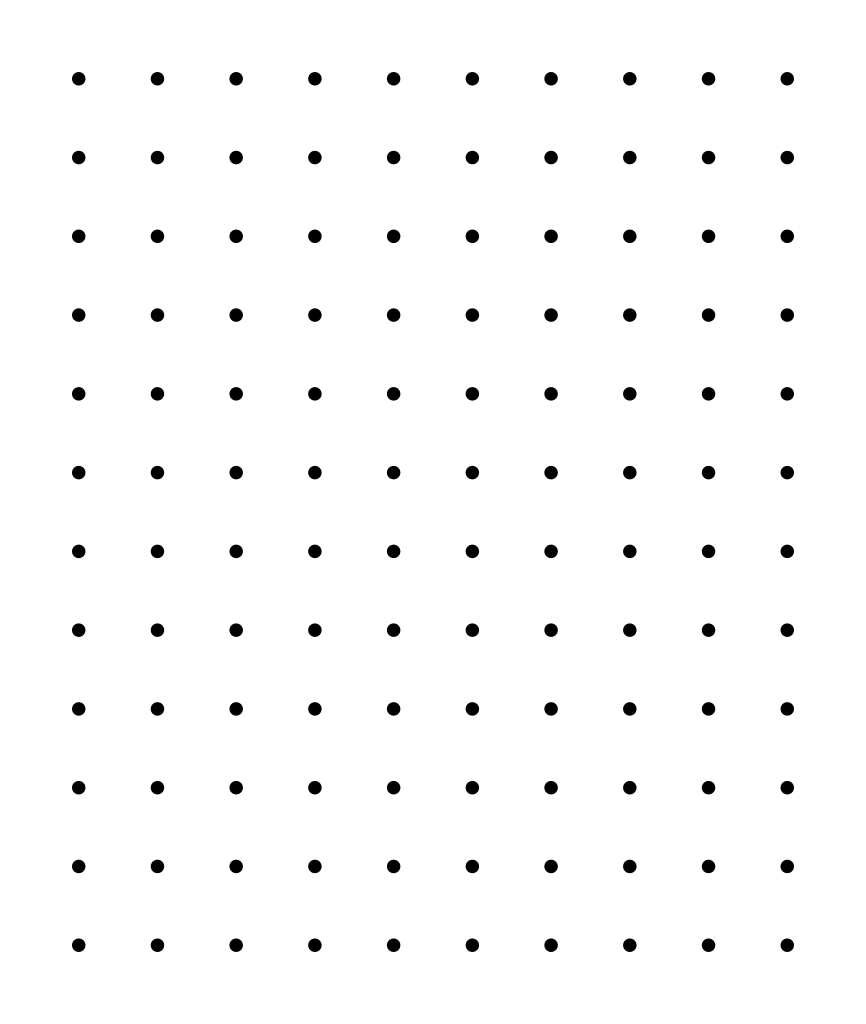
\includegraphics[width=0.75\linewidth]{grid-1}}
      \only<2>{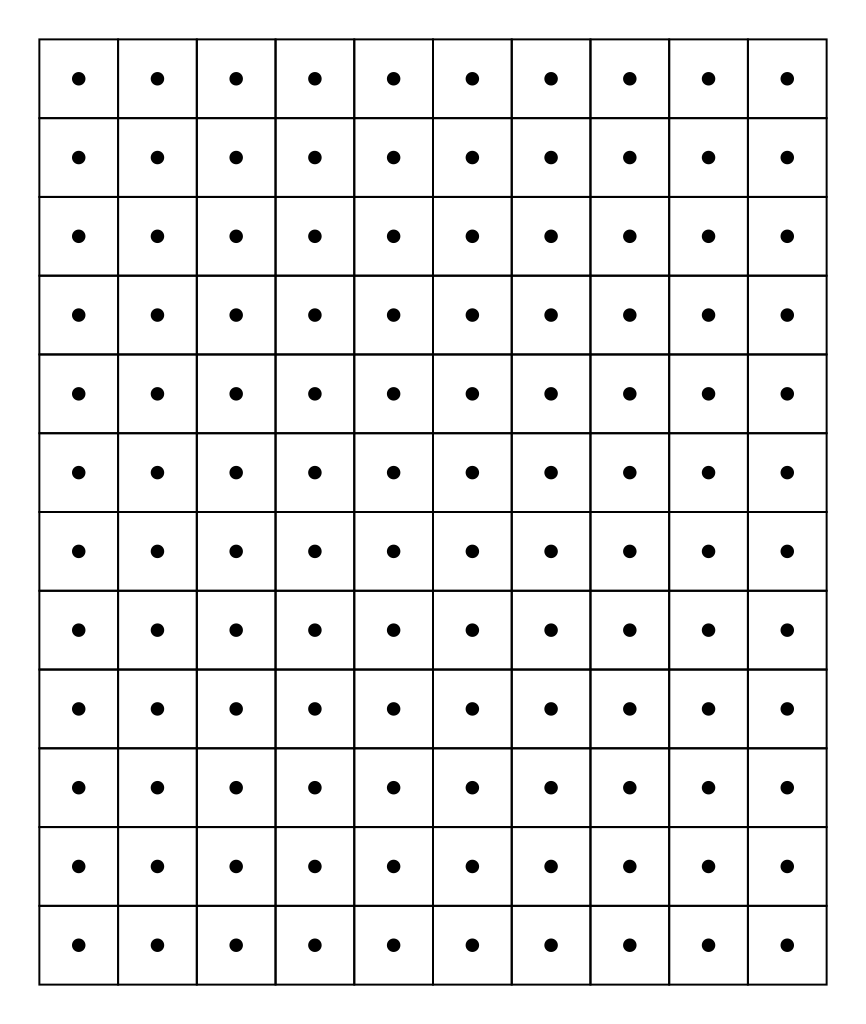
\includegraphics[width=0.75\linewidth]{grid-2}}
      \only<3>{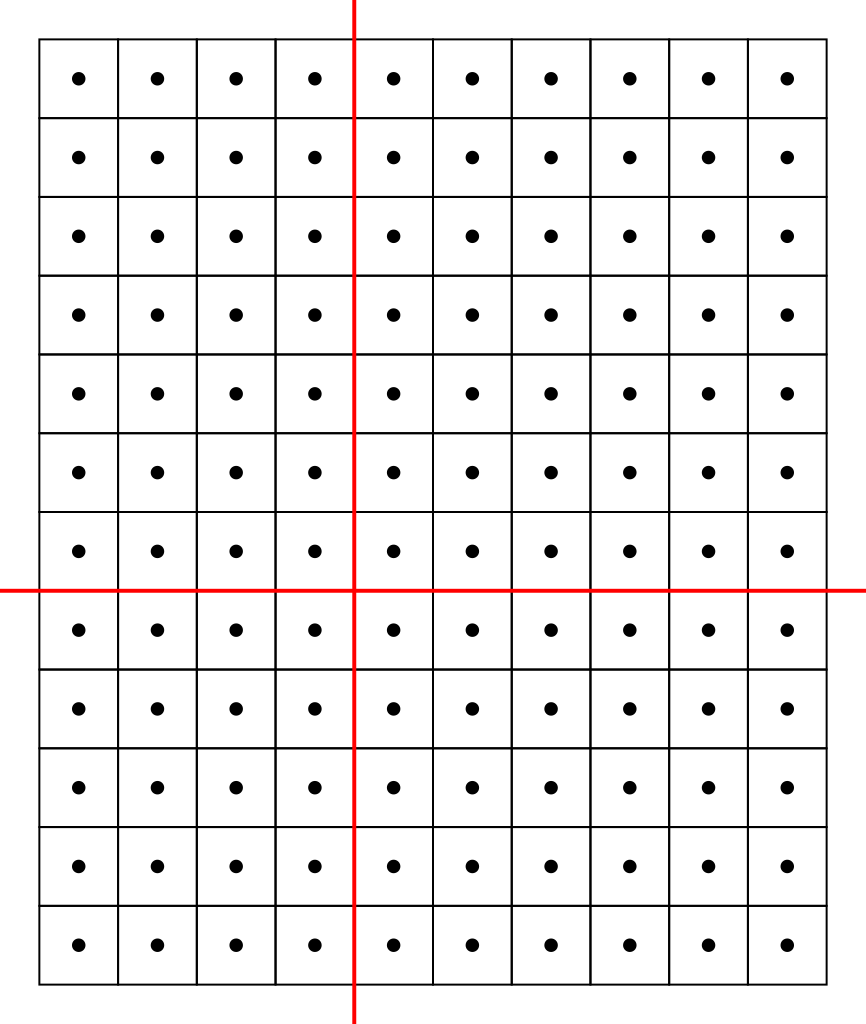
\includegraphics[width=0.75\linewidth]{grid-3}}
      \only<4>{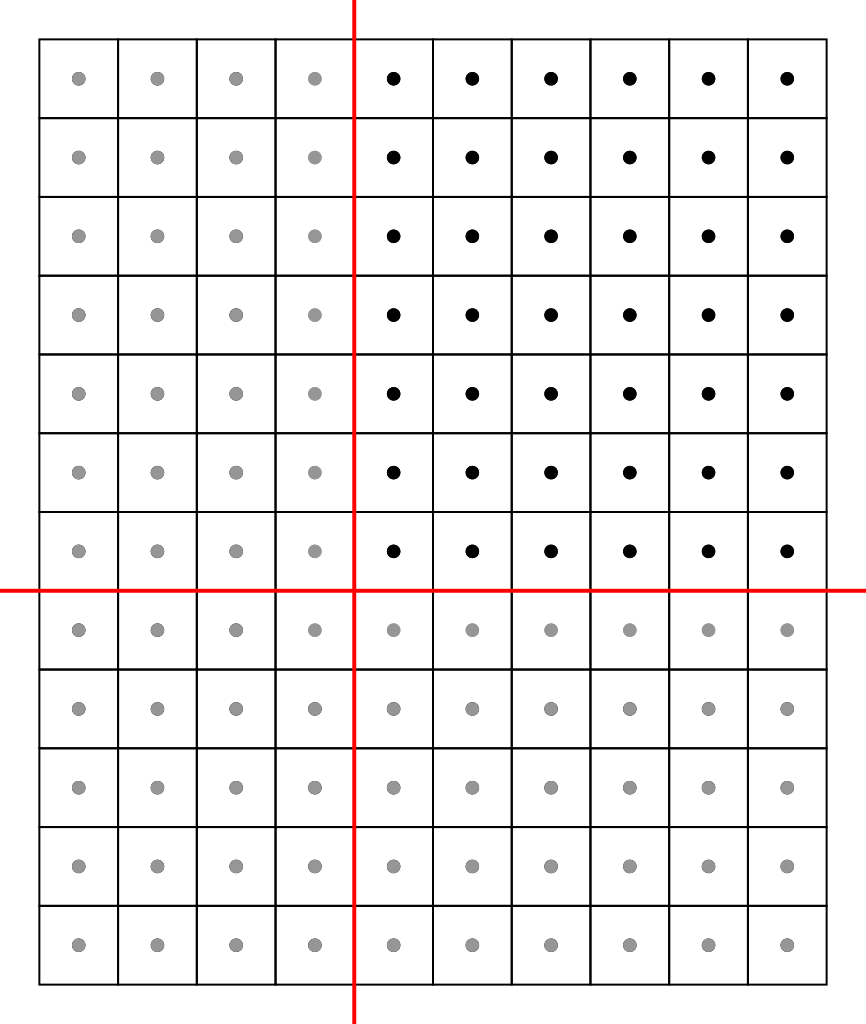
\includegraphics[width=0.75\linewidth]{grid-4}}
      \only<5>{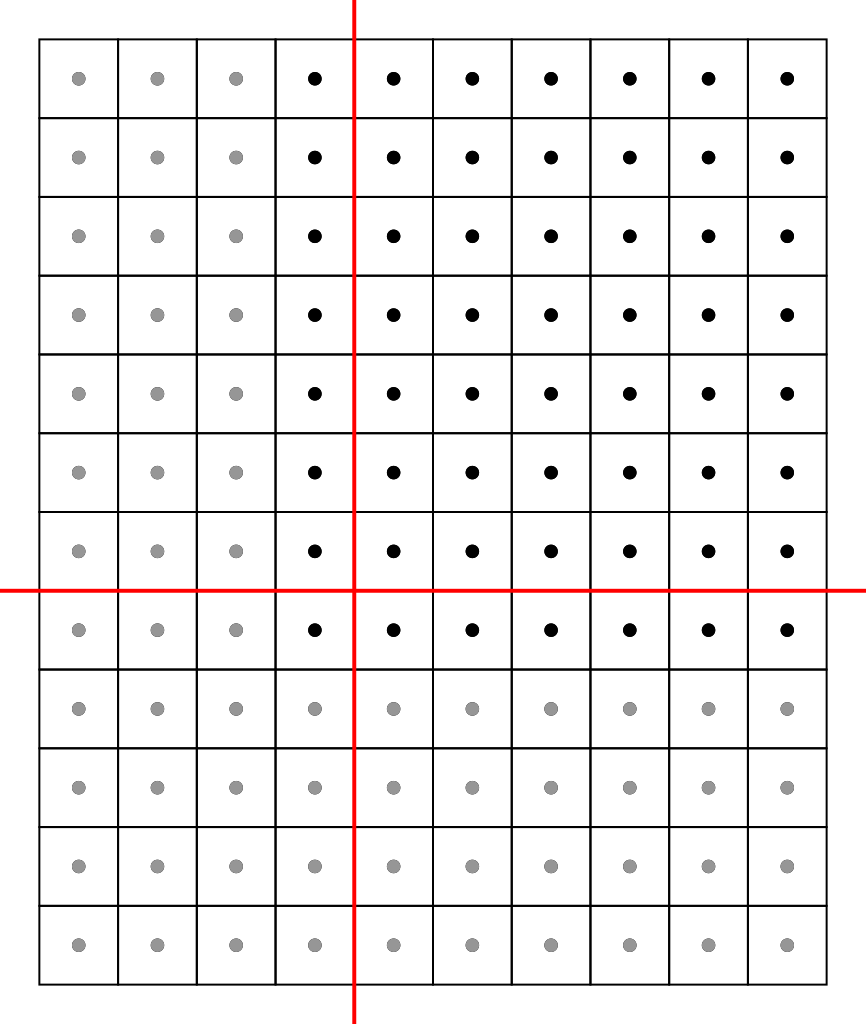
\includegraphics[width=0.75\linewidth]{grid-5}}
    \end{column}
  \end{columns}

\end{frame}

\note{
  The fact that is uses a uniform grid means that it has to
  keep track of more unknowns compared to a model using an
  adaptive mesh, but its output is easier to analyze because it
  does not require post-processing.

  Compute the number of unknowns in a high-ish resolution
  Greenland simulation.

  A figure showing domain decomposition would be useful.

  This is where I would mention ``ghosts'' and that we ne
  ensure that they are up to date, if I thought that it needs
  mentioning.
}

\begin{frame}{Free boundaries}
  Both ice thickness and its extent can change, meaning that PISM has
  to deal with two kinds of free boundaries:

  \begin{itemize}
  \item lateral (in the map plane)
  \item at the top surface
  \end{itemize}
\end{frame}

\note{
  Lateral: a cell is either icy or not, except for ``partially-filled'' cells.
}

\begin{frame}{Free boundary at the top surface and the vertical coordinate}
  There are two common approaches:
  \begin{itemize}
  \item sigma-coordinate
  \item ``immersed'' top boundary plus a transformed vertical
    coordinate
  \end{itemize}
\end{frame}

\begin{frame}
  \frametitle{Vertical sigma coordinate}
  \begin{center}
    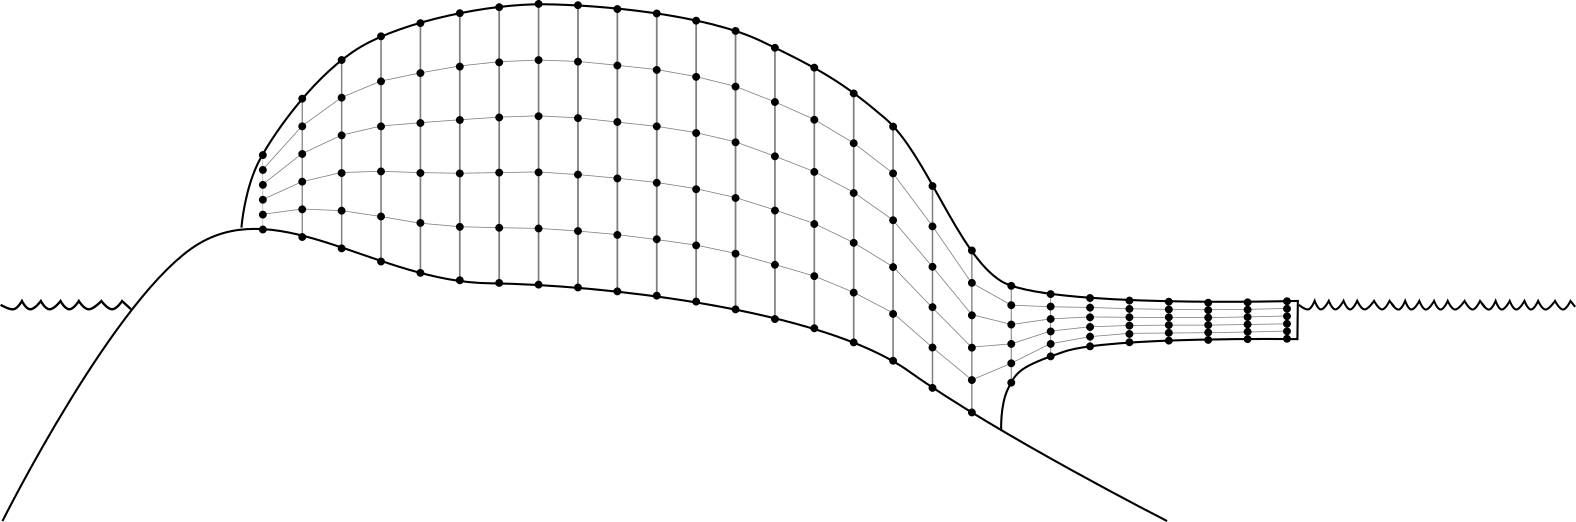
\includegraphics[width=\linewidth]{grid-vertical-sigma}

    \textbf{This approach is used by some other models (e.g. CISM,
      SICOPOLIS), but not by PISM.}
  \end{center}
\end{frame}

\begin{frame}
  \frametitle{PISM's vertical grid}
  \begin{center}
    \only<1>{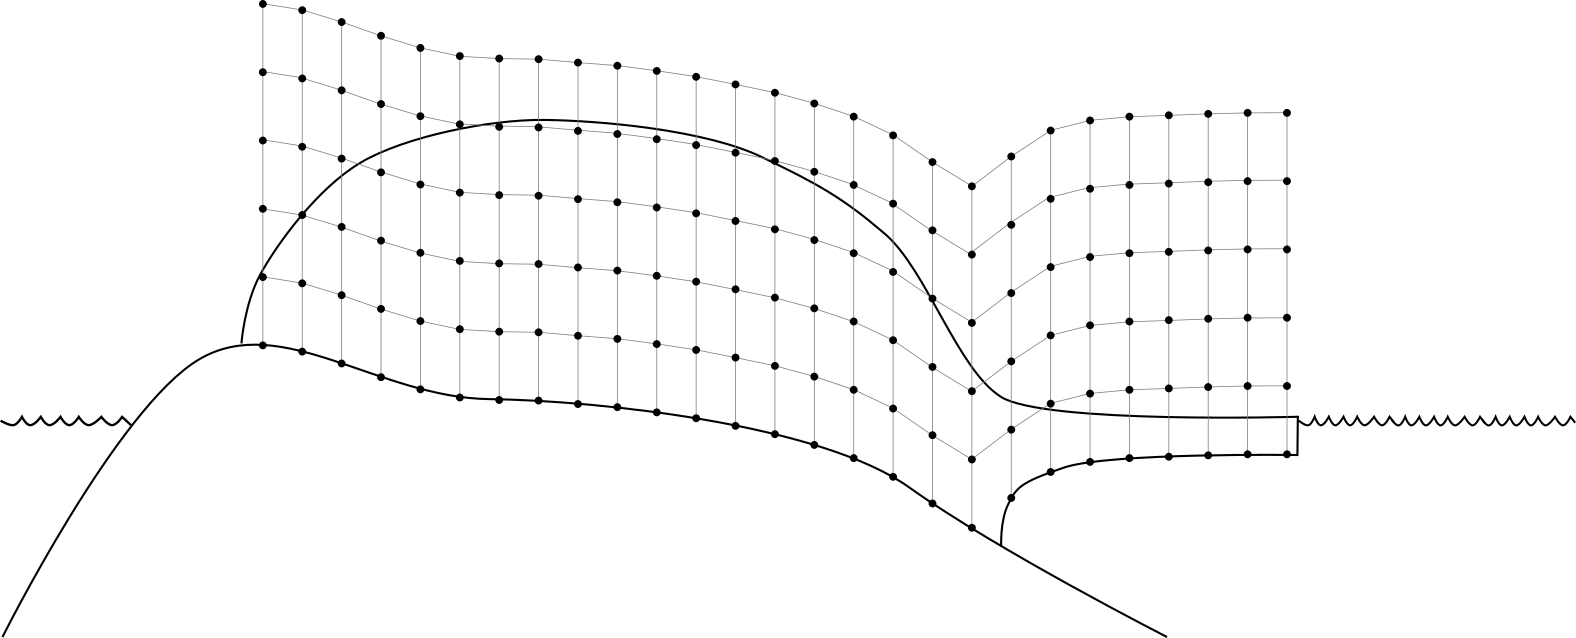
\includegraphics[width=\linewidth]{grid-vertical-pism}}
    \only<2>{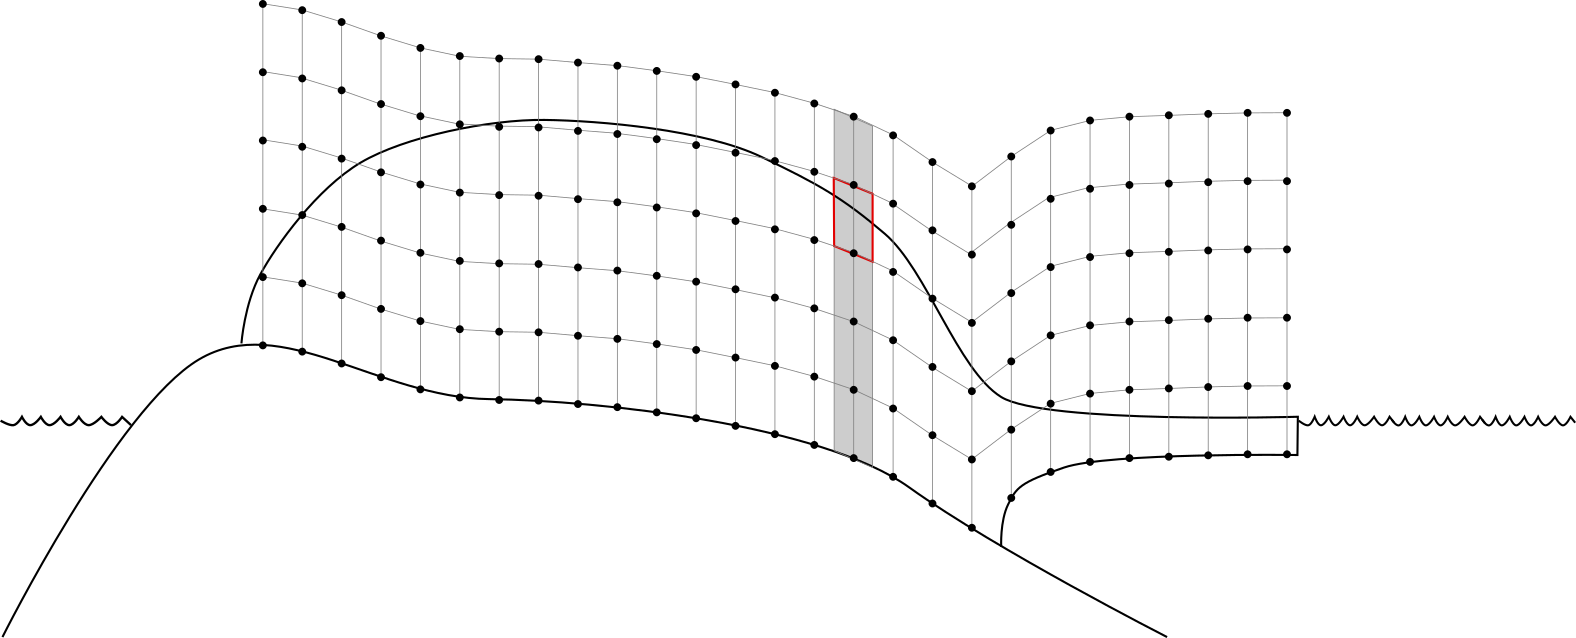
\includegraphics[width=\linewidth]{grid-vertical-pism-boundary}}
  \end{center}
\end{frame}

\note{
  Sigma-coordinate: top boundary follows ice geometry as it
  evolves. Requires modifying most equations (except for shallow,
  two-dimensional ones).

  The surface $z=0$ follows the base of the ice. In general,
  $z=C$ is not a plane; see the Manual for the corresponding
  changes in energy balance equations.
}

\section{Sub-models}
\label{sec:sub-models}

\begin{frame}{Sub-models}

  % PuBu
  \definecolor{levelo}{RGB}{5,112,176}
  \definecolor{leveli}{RGB}{116,169,207}
  \definecolor{levelii}{RGB}{189,201,225}
  \definecolor{leveliii}{RGB}{241,238,246}

  \begin{center}
    \scalebox{0.55}{
      \begin{tikzpicture}[mindmap, concept color=levelo, font=\sf, text=black]

        \tikzstyle{level 1 concept}+=[font=\sf, sibling angle=40]

        \node[concept] {PISM}
        [clockwise from=0]
        child[concept color=leveli]{
          node[concept]{Geometry evolution}
          [clockwise from=60]
          child[concept color=levelii]{ node[concept]{Mass transport} }
          child[concept color=levelii]{ node[concept]{Calving} }
          child[concept color=levelii]{ node[concept]{Iceberg elimination} }
        }
        child[concept color=leveli]{
          node[concept]{Energy balance}
          [clockwise from=-60]
          child[concept color=levelii]{ node[concept]{Bedrock thermal layer}}
        }
        child[concept color=leveli]{ node[concept]{Stress balance} }
        child[concept color=leveli]{ node[concept]{Bed deformation} }
        child[concept color=leveli]{ node[concept]{Age} }
        child[concept color=leveli]{ node[concept]{Subglacial hydrology} }
        child[concept color=leveli]{ node[concept]{Sea level forcing} }
        child[concept color=leveli]{ node[concept]{Sub-shelf boundary conditions} }
        child[concept color=leveli]{
          node[concept]{Top surface boundary conditions}
          [clockwise from=60]
          child[concept color=levelii]{ node[concept]{Atmosphere model} }
        }
        ;
      \end{tikzpicture}
    }                           %scalebox
  \end{center}
\end{frame}

\note{
  These are the parts PISM consists of, conceptually.
}

\begin{frame}{Universal considerations}
  \begin{itemize}
  \item inputs and outputs
  \item initialization
  \item ``bootstrapping'' (initialization from incomplete input data)
  \item time stepping restrictions
  \item computational costs
  \item modeling challenges
  \end{itemize}
\end{frame}

\section{Time stepping}
\label{sec:time-stepping}

\begin{frame}{Explicit time stepping}

  \begin{enumerate}
  \item use stress balance to compute velocity
    \begin{itemize}
    \item often: first get $(u,v)$, then $w$ from incompressibility
    \end{itemize}
  \item somewhere in here do other processes: thermodynamics, basal melt, calving, \dots
  \item decide on time-step $\Delta t$ from diffusivity $D$ \hfill (\emph{or: fixed} $\Delta t$)
  \item from velocity, surface balance, and base balance do time-step of mass continuity equation to get $H_t$
  \item update surface elevation: $h \gets h+H_t \Delta t$
  \item repeat at 1.
  \end{enumerate}

  \bigskip
  \begin{itemize}
  \item this paradigm \emph{is} explicit time stepping of the whole model
  \end{itemize}
\end{frame}

\begin{frame}{PISM's time step}
  Update...
  \begin{enumerate}
  \item basal yield stress
  \item stress balance (ice velocities)
  \item the time step length using stability criteria
  \item age of the ice
  \item energy balance
  \item ice geometry due to flow
  \item sea level
  \item sub-shelf boundary conditions
  \item top-surface boundary conditions
  \item ice geometry due to surface and basal mass balance
  \item subglacial hydrology
  \item bed deformation
  \end{enumerate}
\end{frame}

\section{Stress balance}
\label{sec:stress-balance}

\begin{frame}{Stress balance}
  General organization of PISM's stress balance code (sliding +
  deformation -> (u,v)), the hybrid, $w$ through incompressibility.

  Rheology: Glen-type flow laws \emph{that have a viscosity form}.

  Inputs and outputs (important!).
\end{frame}

\note{

  Note to self: double-check that our strain heating computation is
  correct: should use $w$, not $w_{\text{rel}}$.

}

\subsection{SIA}
\label{sec:sia}

\begin{frame}{Shallow ice approximation (SIA)}

  \begin{align}
    \label{eq:2}
    \frac{\partial H}{\partial t} &= S - \nabla \cdot (Q + \mathbf{U}_b H),\\
    Q &= -D \nabla (b + H),\\
    D &= 2\int_b^h F(z)P(z)(h-z)dz.
  \end{align}

  Can be computed at each grid point independently (using neighboring
  points for FD approximations).

\end{frame}

\begin{frame}{Schoof's parameterized bed roughness technique}
  Modifies the diffusivity of the SIA flow.

  Cite Schoof's paper.

  See the User's Manual and C. Schoof. A variational approach to ice
  stream flow. \emph{J. Fluid Mech}., 556:227–251, 2006 for details.
\end{frame}

\subsection{SSA}
\label{sec:ssa}

\begin{frame}{Shallow shelf approximation (SSA)}

  \begin{align}
    -\left[ 2\bar\nu H\left( 2u_{x} + v_{y}\right)\right]_{x} - \left[\bar\nu
    H\left(u_{y}+v_{x} \right) \right]_{y} - \tau_{(b)1} &= - \rho gH h_{x} \\
    -\left[ \bar\nu H\left( u_{y} + v_{x} \right)\right]_{x} - \left[2\bar\nu
    H\left(u_{x}+2v_{y}  \right) \right]_{y} - \tau_{(b)2} &= -\rho gH h_{y}
  \end{align}

  Here both $\bar \nu$ and $\tau_{b}$ are functions of the ice velocity.

  Boundary conditions at lateral boundaries:
  \begin{equation}
    \label{eq:5}
    \left.t\right|_{\text{cf}} \cdot \mathbf{n} = -p_{\text{o}} \mathbf{n}.
  \end{equation}

  Note: basal (sliding) velocity is \emph{not} prescribed.

\end{frame}

\note{

  FIXME: talk about grounding line transition (``grounded cell
  fraction'').

}

\begin{frame}
  \frametitle{SSA: implementation details}

  PISM uses Picard iteration to solve the non-linear system
  corresponding to the discretization of the SSA system of equations:

  \begin{equation}
    \label{eq:4}
    A(U^{(k)}) U^{(k+1)} = b.
  \end{equation}

  Mention that the system solved by PISM has the same size independent
  from the current ice extent (trivial equations).

  Challenges:
  \begin{itemize}
  \item stopping criterion
  \item robustness
  \item computational cost
  \end{itemize}
\end{frame}

\begin{frame}
  \frametitle{SSA: an alternative implementation approach}

  Mention the alternative (Newton iteration in the FEM
  implementation). Mention challenges of implementing the FEM solver:
  domain shape.

\end{frame}

\begin{frame}
  \frametitle{Basal sliding laws}

  \begin{itemize}
  \item Coulomb

    \begin{equation}
      \label{eq:11}
      |\boldsymbol{\tau}_b| \le \tau_c \quad \text{and} \quad \boldsymbol{\tau}_b =
      - \tau_c \frac{\mathbf{u}}{|\mathbf{u}|} \quad\text{if and only if}\quad |\mathbf{u}| > 0.
    \end{equation}
  \item Pseudo-plastic
  \begin{equation}
    \label{eq:10}
    \boldsymbol{\tau}_b =  - \tau_c \frac{\mathbf{u}}{u_{\text{threshold}}^q |\mathbf{u}|^{1-q}},
  \end{equation}
  \end{itemize}
\end{frame}

\begin{frame}{Basal yield stress models}
  \begin{itemize}
  \item Mohr-Coulomb
  \item constant
  \end{itemize}

  Talk about inputs and outputs, tying this to hydrology.
\end{frame}

\begin{frame}
  \frametitle{Grounding line treatment}

  \only<1>{
    \begin{center}
      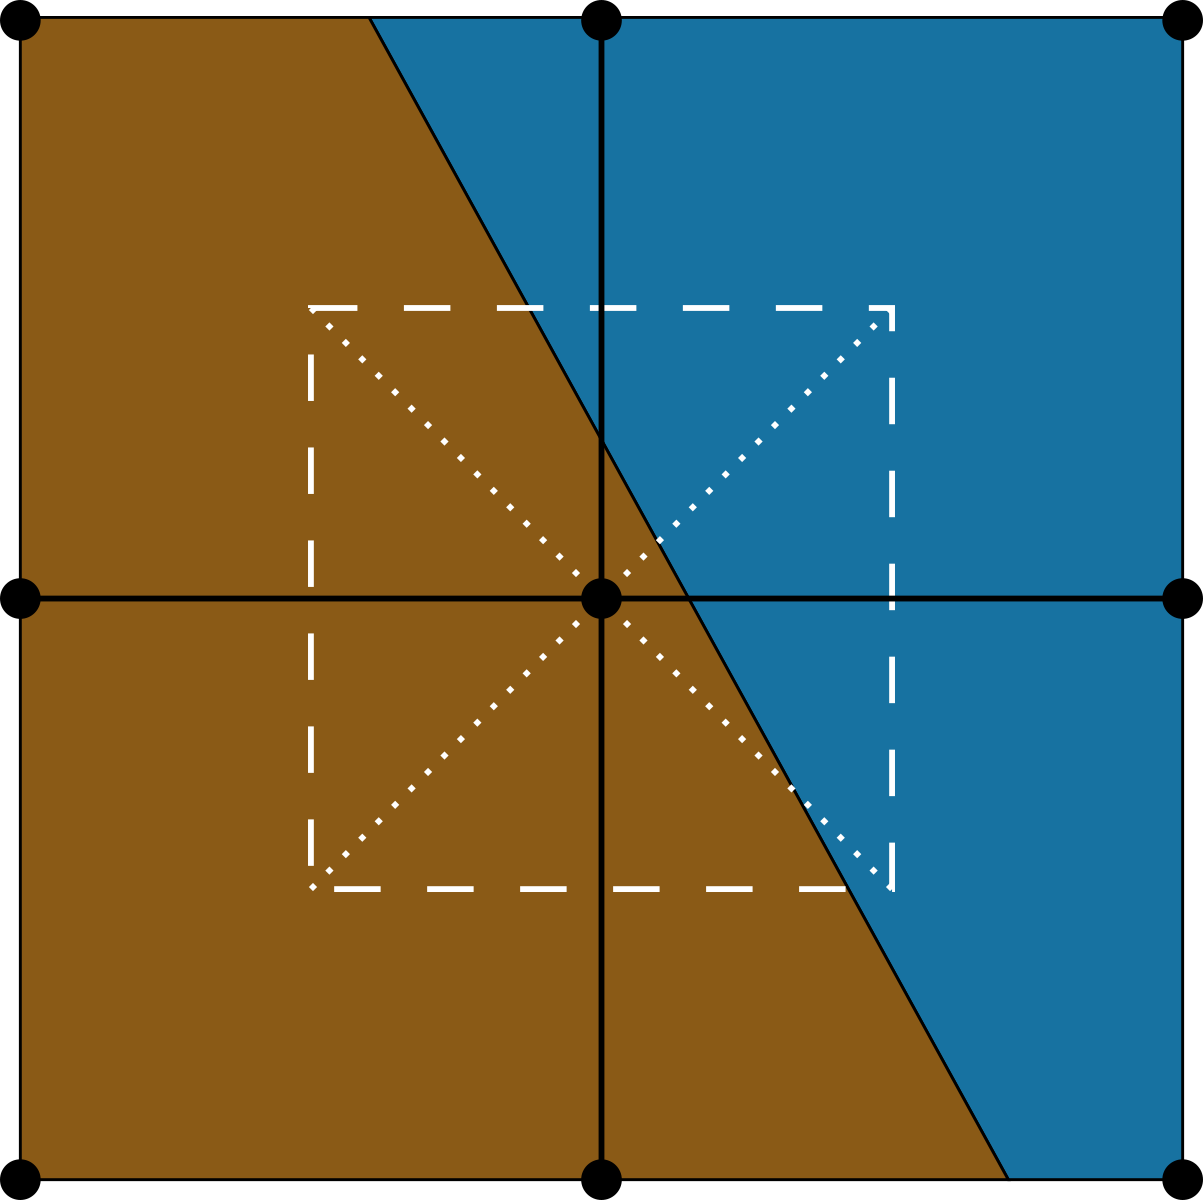
\includegraphics[width=0.4\linewidth]{grounded-cell-fraction}
    \end{center}
  }

  \only<2>{
    ... very similar to SEP1 in \emph{Hydrostatic grounding line
      parameterization in ice sheet models} by Seroussi et al.

    \begin{center}
      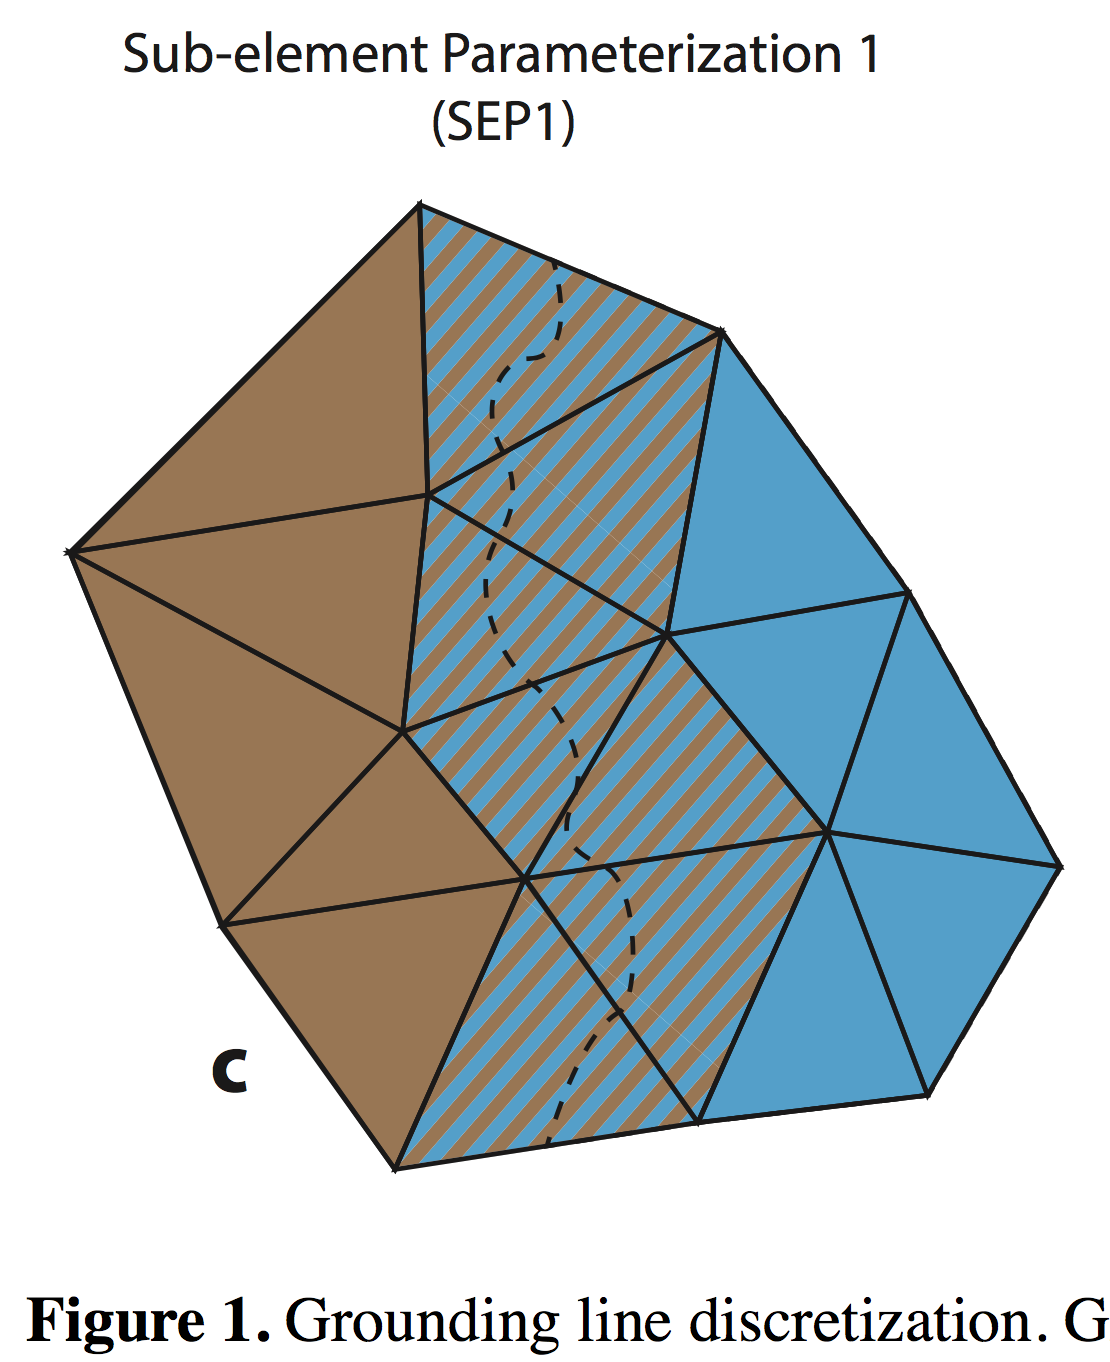
\includegraphics[width=0.4\linewidth]{Seroussi-SEP1}
    \end{center}
  }

\end{frame}

\section{Energy balance}
\label{sec:energy-balance}

\begin{frame}{Energy balance in the ice volume}
  \begin{itemize}
  \item \emph{shallow} conduction-advection equation
    \begin{equation}
      \label{eq:1}
  \rho_{i} \left( \diff{E}{t} + w\,\diff{E}{z} \right) - \diff{}{z}\left( K(E) \diff{E}{z} \right) = Q - \rho_{i} \left( u\,\diff{E}{x} + v\,\diff{E}{y} \right).
    \end{equation}
  \item non-linear conductivity (function of enthalpy)
  \item implicit in the vertical dimension, explicit in horizontal
  \item first order upwinding for advecion
  \item has a CFL time step restriction using 3D $u$ and $v$
    components of the ice velocity
  \end{itemize}
\end{frame}

\note{
  Mention the legacy model: temperature-based energy conservation.

  Mention Aschwanden et al.

  Talk about inputs and outputs, drainage.

  Mention PISM's vertical coordinate.

  Mention (or maybe add a slide about) initialization difficulties:
  spinups, heuristics, data assimilation.

}

\begin{frame}{Energy balance: boundary conditions}

  \begin{columns}[c]
    \begin{column}{0.5\linewidth}
      \begin{itemize}
      \item top: Dirichlet
      \item bottom: Dirichlet or Neumann
      \end{itemize}
    \end{column}

    \begin{column}{0.5\linewidth}
      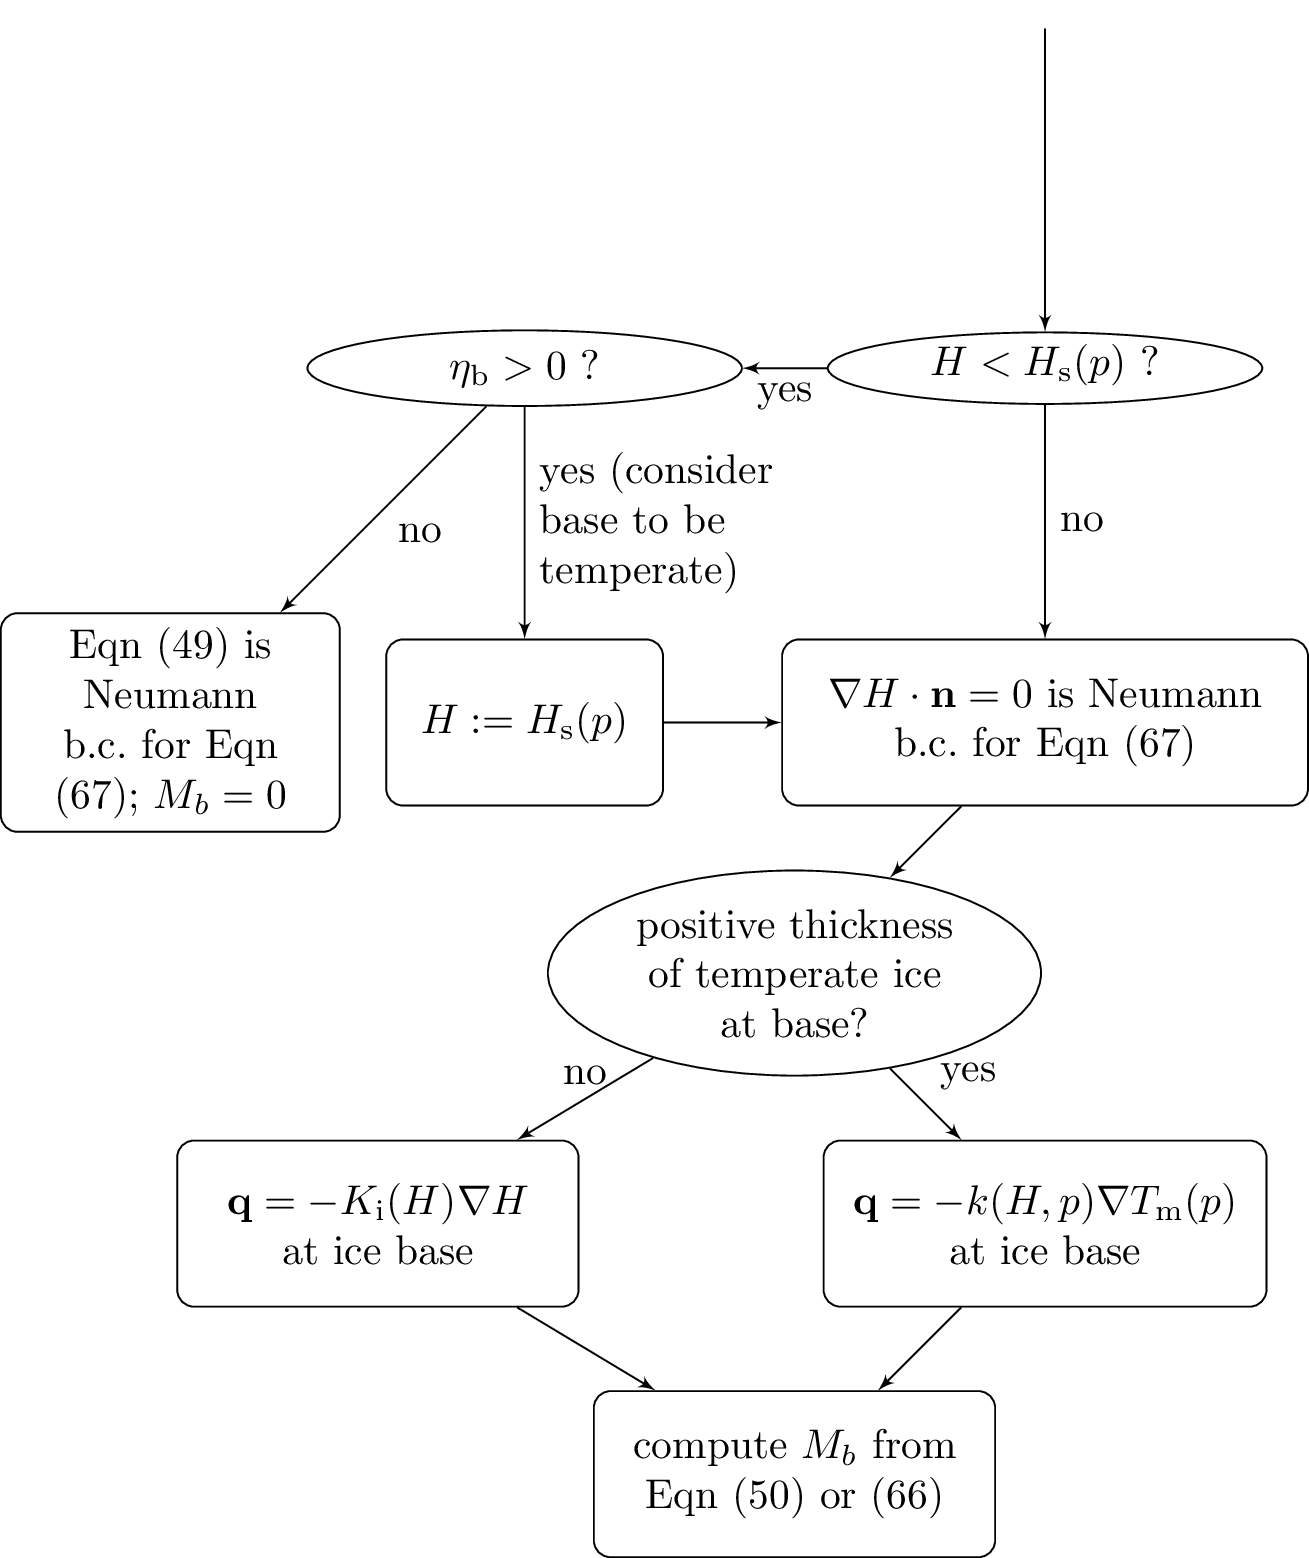
\includegraphics[width=0.9\linewidth]{enthalpy-basal-bc}
    \end{column}
  \end{columns}
\end{frame}

\subsection{Bedrock thermal layer}
\label{sec:bedrock}

\begin{frame}{Bedrock thermal layer}
  Models the temperature in a thin ($\tilde 1000$ km) layer a the top
  of the Earth's crust.

  \begin{itemize}
  \item Assumes that this layer is \emph{shallow}: horizontal
    conduction terms are ignored, i.e. columns of bedrock are treated
    as independent.
  \item Uses a regular grid in bedrock columns, fully implicit, no
    time-step restriction.
  \end{itemize}
\end{frame}

\note{
  The bedrock thermal layer has the largest effect in simulations
  with moving boundaries: edges of ice streams, grounding lines, and
  grounded margins.

  FIXME: talk about inputs and outputs.
}

\section{Geometry evolution}
\label{sec:geometry-evolution}

\begin{frame}{Mass transport}
  \begin{itemize}
  \item uses the finite-volume approach
  \item tailored to take advantage to PISM's split between
    ``diffusive'' and ``advective'' ice flow
  \item ice flow is diffusive, so numerical diffusivity does not cause
    much trouble
  \item surface and basal mass balance may be negative and extra care
    is needed to preserve non-negativity of ice thickness
  \end{itemize}
\end{frame}

\note{ Alternative: coupled stress balance and mass continuity with an
  inequality constraint, i.e. the variational inequality formulation.
}

\begin{frame}{Stability considerations}
  The SIA flow is diffusive, so preserving staility of explicit time
  stepping forces us to respect diffusion-related time step
  restrictions.

  Recall that
  \begin{align}
    \label{eq:2}
    \frac{\partial H}{\partial t} &= S - \nabla \cdot (Q + \mathbf{U}_b H),\\
    Q &= -D \nabla (b + H).\\
  \end{align}

  This applies to other models, even if they don't use the shallow ice
  approximation.

  \begin{equation}
    \label{eq:3}
    \Delta t \le \cdot \Delta x^{2} / D_{\text{max}}.
  \end{equation}

  First-order upwinding for the advective part of the flux gives
  \begin{equation}
    \label{eq:6}
    \Delta t \le 1 / ()
  \end{equation}
\end{frame}

\begin{frame}{Free boundary at the calving front}
  \begin{center}
    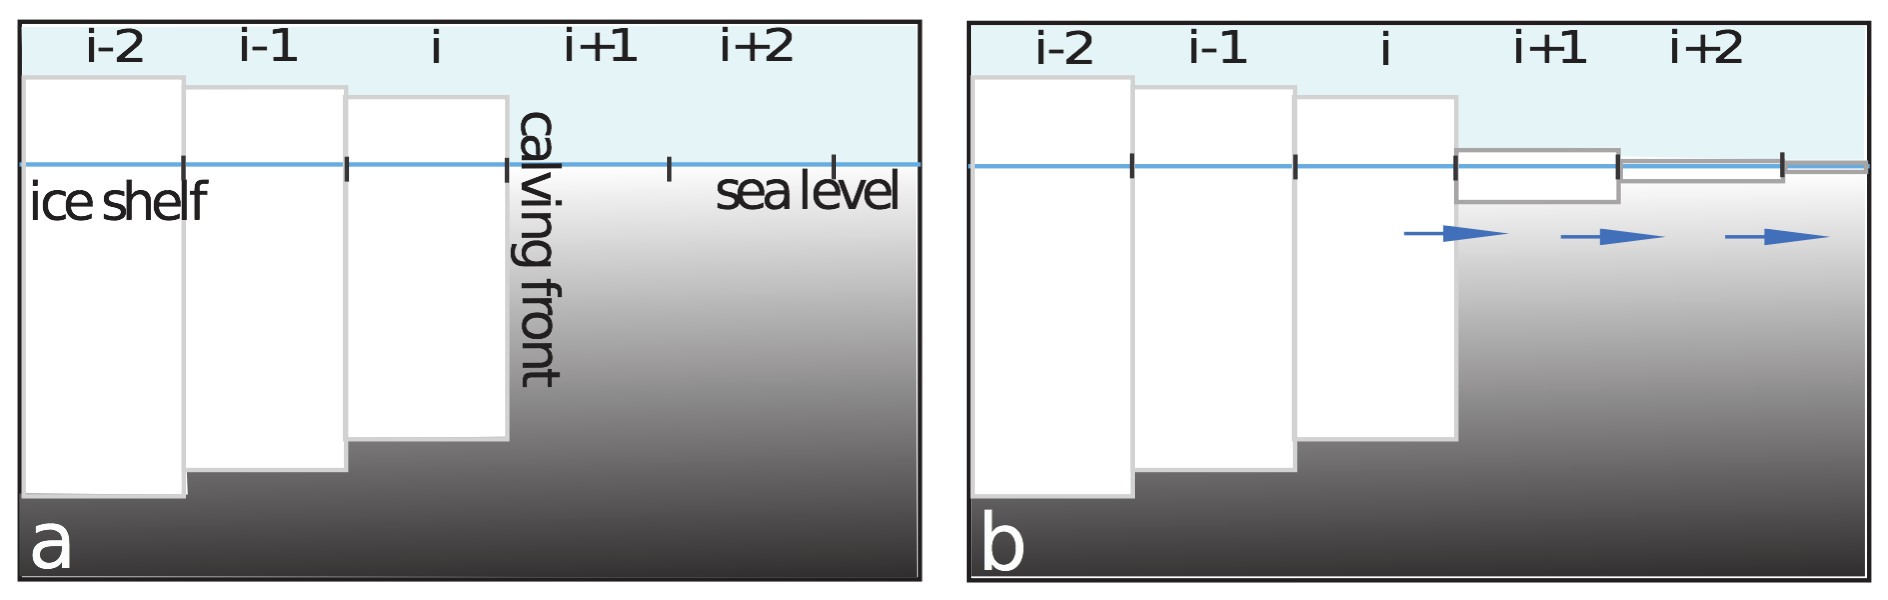
\includegraphics[width=0.8\textwidth]{albrecht-martin-figure-1}

    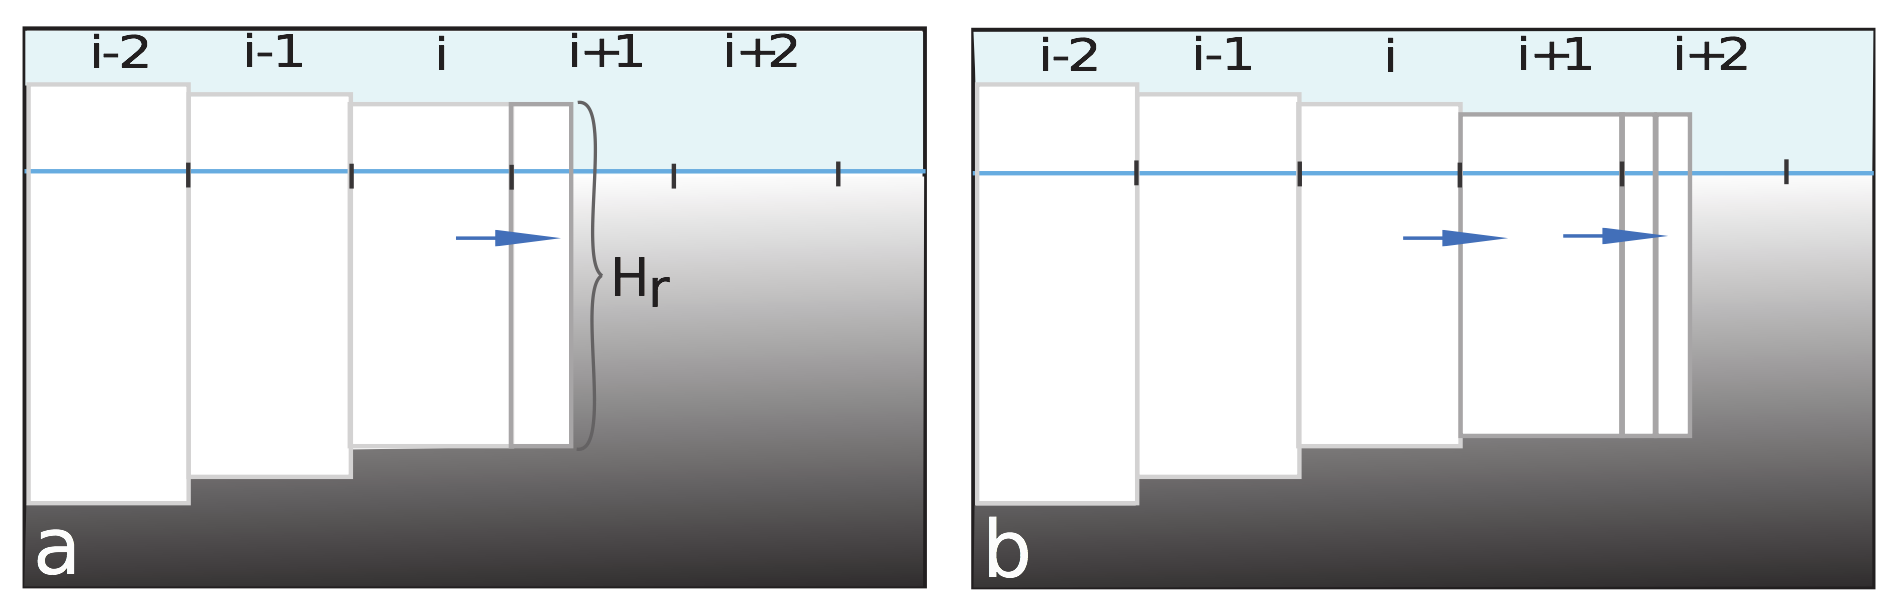
\includegraphics[width=0.8\textwidth]{albrecht-martin-figure-2}
  \end{center}

  See T. Albrecht, M. Martin, M. Haseloff, R. Winkelmann, and A.
  Levermann. Parameterization for subgrid-scale motion of ice-shelf
  calving fronts. \emph{The Cryosphere}, 5:35–44, 2011 for details.
\end{frame}

\subsection{Calving}
\label{sec:calving}

\begin{frame}{Calving}
  \begin{itemize}
  \item Geometric criteria
    \begin{itemize}
    \item ice thickness threshold
    \item floating ice
    \item prescribed maximum shelf extent
    \end{itemize}
  \item Stress-based
    \begin{itemize}
    \item Eigen calving
      \begin{equation}
        \label{eq:7}
        c = K\; \dot{\epsilon}_{_+}\; \dot{\epsilon}_{_-}\quad\text{and}\quad\dot{\epsilon}_{_\pm}>0\:.
      \end{equation}
      See \emph{Kinematic first-order calving law implies
      potential for abrupt ice-shelf retreat} by Levermann et al.
    \item von Mises
      \begin{equation}
        \label{eq:8}
        c = |\mathbf{u}| \frac{\tilde{\sigma}}{\sigma_{max}},
      \end{equation}
      See \emph{Modeling of Store Gletscher’s calving dynamics, West
        Greenland, in response to ocean thermal forcing.} by Morlighem
      et al.
    \end{itemize}
  \end{itemize}
\end{frame}

\note{

  Challenges: strain rates estimated using finite differences may be
  of poor quality.
}

\subsection{Iceberg elimination}
\label{sec:iceberg-elimination}

\begin{frame}{Iceberg elimination}
  Why do we need this?

  \begin{itemize}
  \item The SSA stress balance determines the sliding velocity of
    patches of floating ice \emph{up to rigid body motions} (see C.
    Schoof, \emph{A variational approach to ice stream flow})
  \item We need to keep track of an ice sheet's discharge into the
    ocean.
  \end{itemize}

  Where would an ``iceberg'' (isolated patch of floating ice) come
  from?
  \begin{itemize}
  \item calving
  \item sea level changes
  \end{itemize}
\end{frame}

\begin{frame}{Iceberg elimination: technical details}

  \begin{center}
    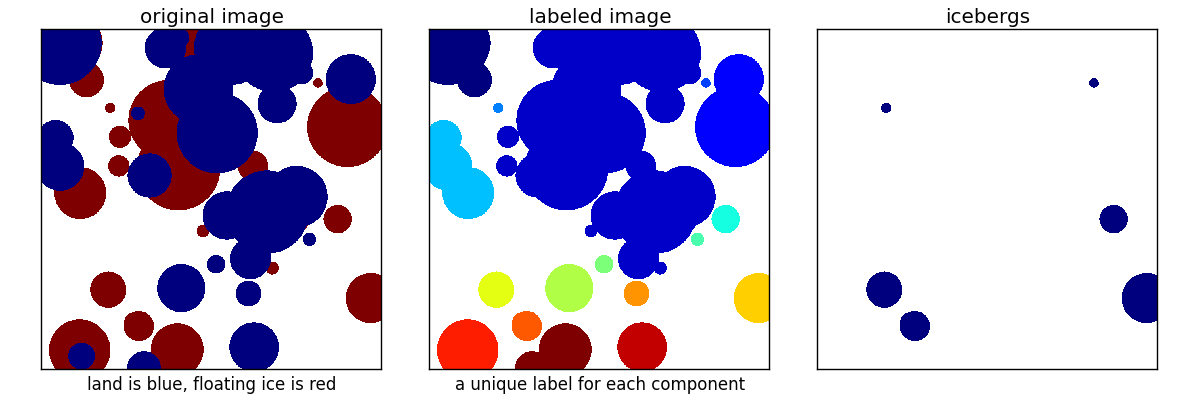
\includegraphics[width=0.9\textwidth]{icebergs.png}
  \end{center}

  \begin{itemize}
  \item uses a 2-scan connected component labeling algorithm (serial code)
  \item computationally cheap
  \end{itemize}
\end{frame}

\section{Bed deformation}
\label{sec:bed-deformation}

\begin{frame}{Bed deformation}
  \begin{itemize}
  \item pointwise isostasy
    \begin{equation}
      \label{eq:9}
      b(t,x,y) = b(0,x,y) - f \left[H(t,x,y) - H(0,x,y)\right].
    \end{equation}
  \item Lingle-Clark model (elastic plate lithosphere over viscous
    half-space plus purely-elastic, spherical, layered,
    self-gravitating earth)

    \medskip
    Only the first component (elastic plate lithosphere over viscous
    half-space) is used in most of simulations.
  \end{itemize}

  FIXME: Inputs, outputs, time scale
\end{frame}

\begin{frame}{Lingle-Clark bed deformation model}
  \begin{itemize}
  \item the fundamental equation includes a pseudo-differential
    operator define using Fourier transform
  \item Fourier spectral collocation method with periodic boundaries
    on an extended domain
  \item no time step restriction
  \item can be initialized using measured uplift rates
  \item relatively cheap computationally
  \item serial code
  \end{itemize}

  See E. Bueler, C. S. Lingle, and J. A. Kallen-Brown. Fast
  computation of a viscoelastic deformable Earth model for ice sheet
  simulation. \emph{Ann. Glaciol}., 46:97–105, 2007
\end{frame}

\section{Environmental forcing}
\label{sec:environment}

\begin{frame}{Environmental forcing}
  Sub-models providing boundary ``climatic''

  \begin{itemize}
  \item Top surface
  \item Bottom surface
  \item Shelf base
  \item Sea level
  \end{itemize}
\end{frame}

\note{FIXME: I need to say more about this.}

\section{Age}
\label{sec:age}

\begin{frame}{Age}
  Numerical diffusivity is a concern.

  Implementation details are the same as in the energy balance code.

  Boundary conditions: 0 at the top surface and at the bottom surface
  with freezing conditions.
\end{frame}

\section{Subglacial hydrology}
\label{sec:subglacial-hydrology}

\begin{frame}{Subglacial hydrology}

  \begin{itemize}
  \item ``Null'' transport: water stored in till, no water conservation
  \item ``Routing'' model: water is stored in till; excess is
    transported along pressure gradient (water pressure assumed equal
    to overburden)
  \item ``Distributed'' model: same as ``routing,'' but with a
    physical model of the water pressure
  \end{itemize}
\end{frame}

\begin{frame}{Subglacial hydrology: challenges}
  \begin{itemize}
  \item vastly different time scale compared to ice flow
  \item poorly constrained model parameters (observations are sparse)
  \item the theory is not mature (no \emph{continuum} model of
    subglacial water transport in channels)
  \end{itemize}
\end{frame}

\note{

  Cite Ed's paper.

}

\end{document}